\chapter{Experiment and Evaluation - System Performance}
\section{Goals}
This experiment is just a proof of concept to show that Graphy's data models for tags and relationships can be exchanged and synchronized between mobile clients like other Contacts application with similar performance. The goals of the experiment are as follows:

\begin{itemize}
    \item Clients can push contact data to backend server.
    \item Clients can pull contact data from backend server.
    \item Clients can synchronize their contact data with each others (through the help of the backend server).
    \item Clients can resolve contact data conflicts between each others (through the help of the backend server).
\end{itemize}

\section{Experimental Setups}
\subsection{Overview}
The experimental system basically contains three parts: the clients, the backend server, and the communication between them. Everything runs on a Macbook Pro 2012 with the specifications listed in \autoref{tb:specs}. The Macbook provides a Unix-like environment where us can run everything we need easily. However, comparing with a real-world, production system, our setup is slower by a huge margin. To be more specific, we use multi-threading programming in order to simulate multiple devices. For communication, we just run the clients and the backed server on the same local host. This method eliminates the delay of the actual Internet connection so we can focus on examining the synchronization process. Even though we can find better equipments, we decide to run our tests on this slow system, if the experiment yields good results, it means it will work even better on a more powerful environment.

\begin{table}[!ht]
\centering
\caption{System's Specifications}\label{tb:specs}
\begin{tabular}{ | c | l | }
\hline
	Processor & \specialcell{2.5GHz dual-core Intel Core i5\\(Turbo Boost up to 3.1GHz)\\with 3MB L3 cache} \\ \hline
	Memory & 8GB of 1600MHz DDR3 memory \\ \hline
	Storage & 500GB 5400-rpm hard drive \\ \hline
	Operating System & OSX Yosemite v.10.10\\ \hline
\end{tabular}
\end{table}

\subsection{Clients}
The actual fully-featured mobile clients are written in C\# on the Xamarin platform. However, in this experiment to reduce the manual tasks to a minimum we re-write the clients into multiple threads, each thread represents one client. We also discard all the unnecessary code like the user interface and other unrelated functions. The experiment code of clients can be accessed at: \url{https://github.com/NamXH/GraphyClient}, and the fully-functional mobile clients' code can be accessed at: \url{https://github.com/NamXH/GraphyPCL}. As a result, we take full controls of the client threads and we can trigger the synchronization process at any specific moment precisely. Moreover, using the asynchronous programming model with Async and Await in C\# we can run many client threads in parallel to simulate multiple devices being used at the same time. Besides, since we only test the performance of the data synchronization which operates on each user separatedly so for fast prototyping we do not implement authentication in the experiment.

On the other hand, the databases of the clients are carefully implemented for every thread. We also use SQLite which is the same technology as the mobile devices. The details of the database schema can be found in Appendix B. Regarding the Sync Queue, each modification on the database (creating/updating/deleting a business record) is mapped to a row in the Sync Queue table. For instance, a creation is be mapped to a POST request, an update is mapped to a PUT request, and a deletion is mapped to a DELETE request. \autoref{fg:sync_queue} shows some examples of the Sync Queue table.

\begin{figure}[!h]
\begin{centering}
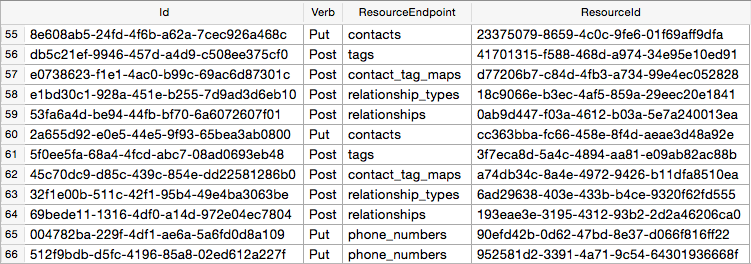
\includegraphics[scale=0.63]{pics/sync_queue.png}
\caption{Sync Queue Table}\label{fg:sync_queue}
\end{centering}
\end{figure}

\subsection{Server}
The backend server is written in Python using the Django framework. Its code can be accessed at: \url{https://github.com/NamXH/GraphyBackend}. \autoref{fg:server_implementation} presents some examples of the database models written for the server. We run the Python code on the Gunicorn web server with 5 workers since our processor has 4 cores. It is also worth mentioning that the server's database is implemented using PostgreSQL - a high performance, open source, relational database. Python and Django have incredible support for PostgreSQL so the setup is very simple. Moreover, we can use the Python object-relational mapper to access PostgreSQL instead of writing raw SQL queries.

\begin{figure}[!h]
\begin{centering}
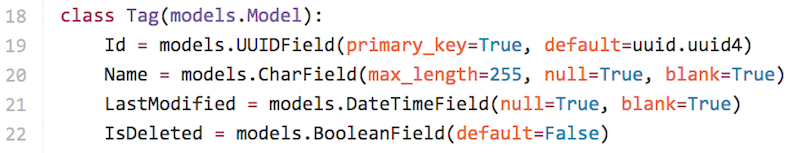
\includegraphics[scale=0.5]{pics/django_tag.png}

\vspace{0.5cm}

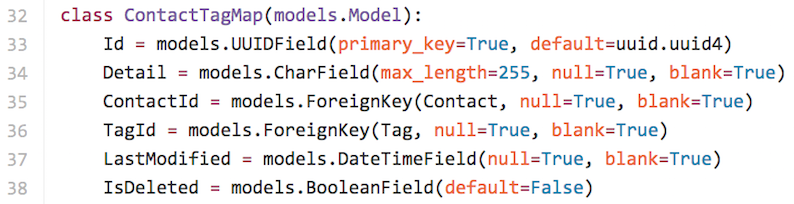
\includegraphics[scale=0.5]{pics/django_tagmap.png}

\vspace{0.5cm}

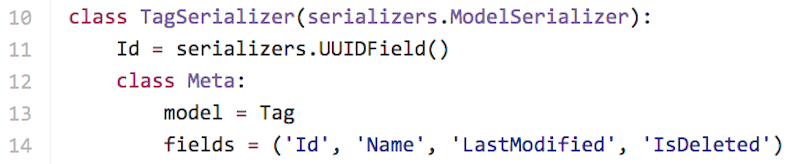
\includegraphics[scale=0.46]{pics/django_serializer.png}
%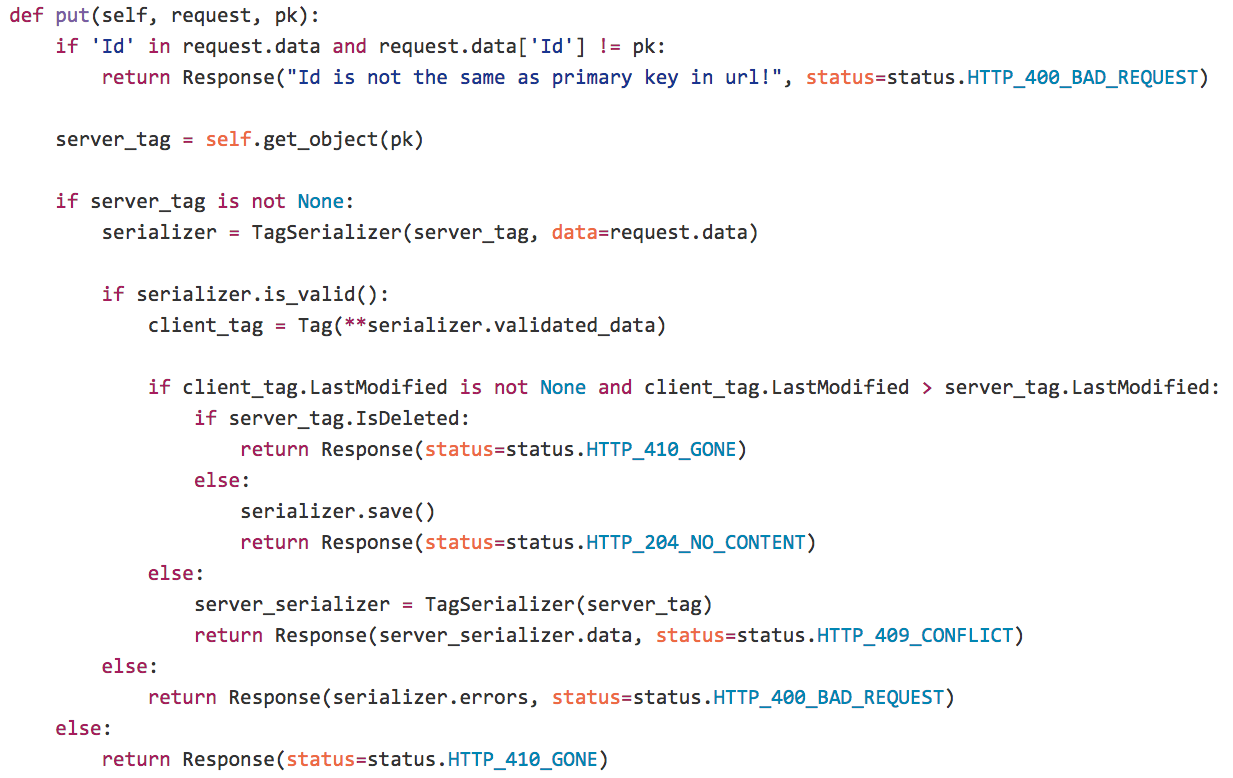
\includegraphics[scale=0.6]{pics/django_put.png}
\caption{Backend Server Implementation}\label{fg:server_implementation}
\end{centering}
\end{figure}


\subsection{Communication}
The communication between the clients and the server is achieved using RESTful HTTP requests. The server provides an API which contains 11 endpoints, each endpoint is corresponded to a table in the database such as contacts, phone numbers, tags, relationships. An endpoint responds to the HTTP requests sent by clients differently to perform the CRUD (Create-Read-Update-Delete) operations on the database. Furthermore, to simulate the intermittent nature of the Internet, we sometimes perform an interruption to the synchronization process. Besides, while many mobile clients are being used by the users, there can be situations that some conflicts occur. Normally, the users have to manually resolve the conflicts. However, to reduce the complexity, we create a time stamp of the last modification on an entry and use it to decide which version to keep (i.e., we keep the latest version).

% To resolve the conflicts, we apply opportunistic locking to our database. The basic idea is maintaining a version for every database entry and only allowing modification if the client's entry has the same version as the server's entry, when the two entries have different versions (conflict) the user has to resolve the conflict manually
% This solution just simplifies the implementation without any significant impact on the synchronization process.

\section{Scenarios and Results}
In order to test whether our system achieves the goals, we ran it through different scenarios and evaluated the results. The default datasets used in every scenario consisted of 200 contacts, each contact had 3 traditional fields: first name, phone number, and email. Additionally, there were also 100 tags attached to 100 contacts, and 100 relationships which connected 100 pairs of contacts. The details of the scenarios will be discussed in the following sections.

\subsubsection{Scenario 1: Creation}
The first scenario aimed at testing the first goal: \textit{Clients can push contact data to backend server}. Therefore, we created an initial database with the default dataset in the client then started the synchronization process. This scenario tried to simulate the situation when a person uses Graphy for the first time in which he/she imports and creates a few contacts then starts the synchronization process when the Internet connection is available. Each creation or importation in Graphy is associated with a row in the database, then each row has a corresponding POST operation in the Sync Queue. It is important to note that before the first synchronization the users may also modify or delete some of their new entries. As a result, the Sync Queue may contain PUT and DELETE operations. However, in Graphy's algorithm instead of creating new PUT or DELETE operations of a new entry we inspect the actions and just modify the corresponding POST operation so there are only one POST operation for every newly created entry.

\subsubsection{Scenario 2: Modification}
The second scenario..

\subsubsection{Scenario 3: Retrieval}
In this scenario..

\subsubsection{Scenario 4: Synchronization}
abc

\subsubsection{Scenario 5: Conflicts Resolution}
abc

\begin{table}[!ht]
\centering
\caption{abc}\label{tb:abc}
\begin{tabular}{ | c | c | c |}
\hline
	Creation/Modification & Retrieval & Gmail Retrieval \\ \hline
	9.59 & 4.03 & 18.47 \\ \hline
	9.75 & 4.58 & 20.77 \\ \hline
	9.85 & 5.03 & 19.73 \\ \hline
	9.49 & 4.30 & 17.92 \\ \hline
	9.57 & 4.63 & 21.81 \\ \hline
	9.63 & 4.99 & 19.89 \\ \hline
	10.11 & 5.00 & 18.32 \\ \hline
	9.59 & 4.21 & 20.59 \\ \hline
	10.50 & 4.88 & 19.29 \\ \hline
	9.79 & 4.90 & 20.07 \\ \hline
        \multicolumn{3}{| l |}{\textit{Average:}} \\ \hline
        \textbf{9.79}& \textbf{4.66} & \textbf{19.69}\\ \hline
\end{tabular}
\end{table}

%\begin{table}[!ht]
%\centering
%\caption{abc}\label{tb:abcd}
%\begin{tabular}{ | c | c | }
%\hline
%	Creation/Modification & Retrieval & Gmail Retrieval \\ \hline
%	9.5877 & 4.0301 & 18.47 \\ \hline
%	9.7471 & 4.5846 & 20.77 \\ \hline
%	9.8455 & 5.0286 & 19.73 \\ \hline
%	9.4878 & 4.2998 & 17.92 \\ \hline
%	9.5682 & 4.6329 & 21.81 \\ \hline
%	9.6295& 4.9852 & 19.89 \\ \hline
%	10.1144 & 5.0014 & 18.32 \\ \hline
%	9.5907 & 4.2031 & 20.59 \\ \hline
%	10.4971 & 4.8837 & 19.29 \\ \hline
%	9.7939& 4.9016 & 20.07 \\ \hline
%        \multicolumn{2}{| l |}{\textit{Average:}} \\ \hline
%        \textbf{9.7861}& \textbf{4.6551} & \textbf{19.686}\\ \hline
%\end{tabular}
%\end{table}

\begin{figure}[!h]
\begin{centering}
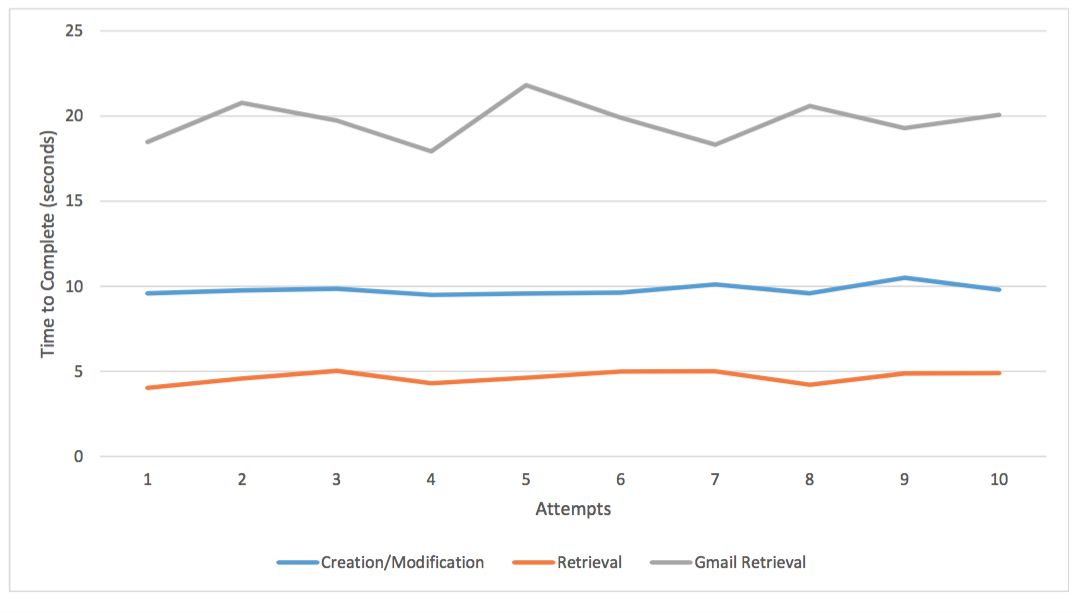
\includegraphics[scale=0.45]{pics/system_performance.png}
\caption{abc}\label{fg:system_performance}
\end{centering}
\end{figure}

\section{Conclusion}
